\subsection{Recurrent Neural Network}

We implemented a recurrent neural network (RNN) model to perform genre classification using movie plot descriptions as input. The model consists of an embedding layer followed by a simple RNN and a fully connected output layer. The embedding layer maps each token in the input sequence to a dense vector representation, and these embeddings are kept static during training. The RNN processes the sequence of embeddings and captures sequential dependencies in the text, and the final hidden state is passed through a linear layer to produce class predictions.

For training, we used the cross-entropy loss function, which is suitable for multi-class classification tasks. The model parameters were optimized using the Adam optimizer with a learning rate of 0.001. The model was trained for a fixed number of epochs, and performance was evaluated on a validation set after each epoch.

In addition to our RNN model, we implemented simple baselines for comparison. The majority baseline predicts the most frequent class for all inputs, while the random baseline assigns labels randomly. These baselines provide a reference point for evaluating whether the model is learning meaningful patterns from the data.

Our RNN model achieved similar accuracy to the majority baseline but significantly improved the weighted F1 score, this can be seen in table \ref{rnn-comparison-results}. This indicates that while the model does not drastically improve overall accuracy, it performs better across multiple classes rather than focusing only on the dominant class. Compared to other models implemented by our group, such as logistic regression and transformer-based approaches, the RNN performed worse in terms of both accuracy and F1 score. This was expected, as RNNs with static embeddings are less expressive than models using pretrained contextual embeddings such as BERT.

One possible reason for this performance gap is that the embeddings used in our model are not pretrained and remain fixed during training, limiting the model's ability to capture deeper semantic relationships. Additionally, the simple RNN architecture may struggle with long sequences and complex language patterns present in movie plot descriptions.

Overall, while the RNN model outperformed simple baselines in terms of F1 score, it did not outperform more advanced models. However, it provides a useful comparison point and demonstrates the importance of representation quality and model complexity in text classification tasks.

\begin{figure}[h]
  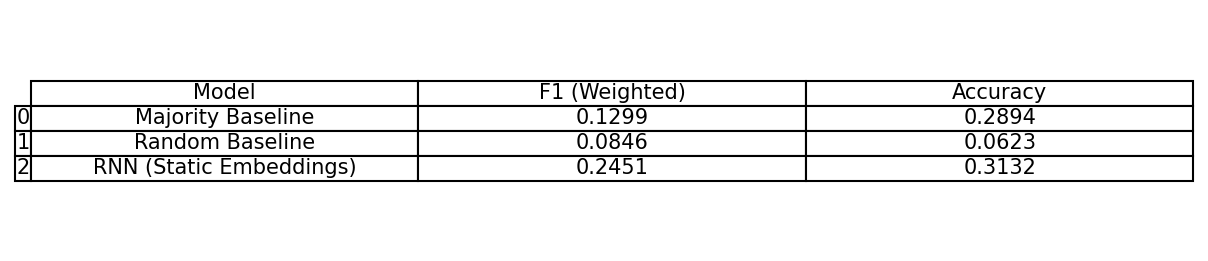
\includegraphics[width=\columnwidth]{../models/rnn/comparison-results.png}
  \caption{Comparison of RNN model performance against baselines.}
  \label{rnn-comparison-results}
\end{figure}